\documentclass[conference]{IEEEtran}
\IEEEoverridecommandlockouts
% The preceding line is only needed to identify funding in the first footnote. If that is unneeded, please comment it out.
\usepackage[hidelinks]{hyperref}
\urlstyle{same}
\usepackage[spanish,es-tabla]{babel}
\usepackage{cite}
\usepackage{amsmath,amssymb,amsfonts}
\usepackage{algorithmic}
\usepackage{graphicx}
\usepackage{textcomp}
\usepackage{xcolor}
\decimalpoint
\renewcommand{\labelitemi}{$\bullet$}
\def\BibTeX{{\rm B\kern-.05em{\sc i\kern-.025em b}\kern-.08em
    T\kern-.1667em\lower.7ex\hbox{E}\kern-.125emX}}
    
    
 %-------------------------------------------------------------------------------
%                            Libreria de codigos                               %
%-------------------------------------------------------------------------------
% Paquetes necesarios
\usepackage{listings}
\usepackage{xcolor}
\usepackage{comment}

% Tipos de letra personalizadas
\def\lstbasicfont{\fontfamily{pcr}\selectfont\scriptsize}
\def\vhdlbasicfont{\fontfamily{cmtt}\selectfont\scriptsize}

% Colores personalizados
\definecolor{codegreen}{rgb}{0,0.6,0}
\definecolor{codepurple}{rgb}{0.58,0,0.82}

\definecolor{codegray}{rgb}{0.5,0.5,0.5}
\definecolor{backcolour}{rgb}{0.95,0.95,0.92}
\definecolor{codeorange}{RGB}{254, 100, 35}

% Deficion de lenguajes perzonalizados

% Definicion de lenguaje MATLAB
\lstdefinelanguage{matlabfloz}{%
  alsoletter={...},%
  morekeywords={%                             % keywords
		break,case,catch,classdef,continue,else,
		elseif,end,for,function,global,if,
		otherwise,parfor,persistent,
		return,spmd,switch,try,while,...},        % Use the matlab "iskeyword" command to get those
  comment=[l]\%,                              % comments
  morecomment=[l]...,                         % comments
  morecomment=[s]{\%\{}{\%\}},                % block comments
  morestring=[m]'                             % strings 
}[keywords,comments,strings]%

% Estilos MATLAB
\lstdefinestyle{MATLAB}{
	frame=single,
	rulecolor=\color{black},
	framexleftmargin=4mm,
	xleftmargin=2mm,
	language=matlabfloz,
  commentstyle=\color{codegreen},
  keywordstyle=\color{blue}, %magenta
  numberstyle=\tiny\color{black},
  stringstyle=\color{codepurple},
  basicstyle=\lstbasicfont\scriptsize,
  breakatwhitespace=false,         
  breaklines=true,                 
  captionpos=b,                    
  keepspaces=true,                 
  numbers=left,                    
  numbersep=5pt,                  
  showspaces=false,                
  showstringspaces=false,
  showtabs=false,                  
  tabsize=2    
}

\lstdefinestyle{PYTHON}{
	frame=single,
	rulecolor=\color{black},
	framexleftmargin=4mm,
	xleftmargin=2mm,
	language=python,
    backgroundcolor=\color{backcolour},   
    commentstyle=\color{codegreen},
    keywordstyle=\color{blue}, %magenta
    numberstyle=\tiny\color{black},
    stringstyle=\color{codeorange},
    basicstyle=\lstbasicfont\footnotesize,
    breakatwhitespace=false,         
    breaklines=true,                 
    captionpos=b,                    
    keepspaces=true,                 
    numbers=left,                    
    numbersep=5pt,                  
    showspaces=false,                
    showstringspaces=false,
    showtabs=false,                  
    tabsize=2,
    otherkeywords = {show,arange}  
}



\lstdefinestyle{BASH}{
	frame=single,
	rulecolor=\color{black},
	framexleftmargin=4mm,
	xleftmargin=2mm,
	language=bash,
    %backgroundcolor=\color{backcolour},   
    commentstyle=\color{codegreen},
    keywordstyle=\color{blue}, %magenta
    numberstyle=\tiny\color{black},
    stringstyle=\color{codeorange},
    basicstyle=\lstbasicfont\footnotesize,
    breakatwhitespace=false,         
    breaklines=true,                 
    captionpos=b,                    
    keepspaces=true,                 
    numbers=left,                    
    numbersep=5pt,                  
    showspaces=false,                
    showstringspaces=false,
    showtabs=false,                  
    tabsize=2,
    %otherkeywords = {show,arange}  
}

\renewcommand{\lstlistingname}{Código}% Listing -> Algorithm
\renewcommand{\lstlistlistingname}{Lista de códigos}% 
\begin{document}

\title{Tarea 4: Optimización multiobjetivo utilizando el algoritmo de NSGA-II para resolver los problemas Osykzka-Kundu y Tanaka
}

\author{\IEEEauthorblockN{Ciro Fabian Bermudez Marquez}
INAOE\\
Mexico, Puebla \\
\url{cirofabian.bermudez@gmail.com}
}

\maketitle

\begin{abstract}
En este trabajo se pone a prueba el algoritmo NSGA-II para resolver los problemas de Osykzka-Kundu y Tanaka.
\end{abstract}



\section{Descripción del problema}

Utilizando el algoritmo de NSGA-II resolver los problemas de Tanaka y Osykzka-Kundu los cuales están codificados en lenguaje C y se presentan en la siguiente sección.


\section{Problema de Tanaka (1995)}
El problema de Tamaka es un problema de dos variables, dos objetivos y dos restricciones definido de la siguiente manera:

Minimizar:
\begin{equation}
f_{1}(\mathbf{x}) = x_{1} \qquad f_{2}(\mathbf{x}) = x_{2}
\end{equation}

Sujeto a:
\begin{equation}
C_{1}(\mathbf{x})  = x_{1}^{2} + x_{2}^{2} - 1 - 0.1 \cos \left(  16 \arctan \frac{x_{1}}{x_{2}}\right) \geq 0  
\end{equation}

\begin{equation}
C_{2}(\mathbf{x})  = (x_{1} -0.5)^{2} + (x_{2} -0.5)^{2}  \leq 0.5 
\end{equation}

\begin{equation}
0 \leq x_{1} \leq \pi \qquad 0 \leq x_{2} \leq \pi
\end{equation}

donde $\mathbf{x} = \left[ x_{1}, x_{2} \right]^{T}$.
\section{Problema de Osyczka-Kundu (1995)}
El problema de Osyczka-Kundu es un problema de seis variables, dos objetivos y 6 restricciones definido de la siguiente manera:

Minimizar:

\begin{align*}
f_{1}(\mathbf{x}) = &  -[ 25 ( x_{1} - 2)^{2} + ( x_{2} - 2)^{2} + ( x_{3} - 1)^{2} \\
    &  + ( x_{4} - 4)^{2} + ( x_{5} - 1)^{2} ]
\end{align*}



\begin{equation}
f_{2}(\mathbf{x}) = x_{1}^{2} + x_{2}^{2} + x_{3}^{2} + x_{4}^{2} + x_{5}^{2} + x_{6}^{2}
\end{equation}



Sujeto a:
\begin{equation}
C_{1}(\mathbf{x})  = x_{1} + x_{2} -2 \geq 0
\end{equation}

\begin{equation}
C_{2}(\mathbf{x}) = 6 - x_{1} -x_{2}   \geq 0
\end{equation}

\begin{equation}
C_{3}(\mathbf{x}) = 2 - x_{2}  + x_{1}   \geq 0
\end{equation}

\begin{equation}
C_{4}(\mathbf{x}) = 2 - x_{1}  + 3 x_{2}   \geq 0
\end{equation}

\begin{equation}
C_{5}(\mathbf{x}) = 4 - (x_{3} -3)^{2} -x_{4}  \geq 0
\end{equation}

\begin{equation}
C_{6}(\mathbf{x}) = (x_{5} -3)^{2} -x_{6}  \geq 0
\end{equation}

\begin{equation}
0 \leq x_{1},x_{2},x_{6} \leq 10  \qquad 1 \leq x_{3}, x_{5}  \leq 5 
\end{equation}

\begin{equation}
0 \leq x_{4} \leq 6
\end{equation}

donde $\mathbf{x} = \left[ x_{1}, x_{2}, \cdots, x_{6} \right]^{T}$.
\section{Resultados}

\subsection{Solución de problema de Tanaka}

Para resolver este problema se utilizaron las semillas mostradas en la Tabla \ref{tab:tanaka} y los siguientes parámetros:

	\begin{table}[!hbp]   
	\caption{Semillas para algoritmo de Tanaka.}                                                                                                                
		\centering                                       
		\begin{tabular}{cc}
			\hline                                             
			Semilla & Valor \\                     
			\hline 
			1 & 0.123\\                                            
			2 & 0.2\\
			3 & 0.3\\
			\hline                                             
		\end{tabular}
		\label{tab:tanaka}
	\end{table}	


\begin{itemize}
\item Tamaño de población: 200
\item Número de generaciones: 300
\item Número de objetivos: 2
\item Número de restricciones: 2
\item Número de variables reales: 2
\item Rango de la variable $x_{1}$: $[ 0,3.15]$
\item Rango de la variable $x_{2}$:  $[ 0,3.15]$
\item Probabilidad de cruza: 0.9
\item Probabilidad de mutación: 0.5
\item Índice de distribución para el cruce SBX variable real $\eta_{c}$:   5 
\item Índice de distribución para la mutación polinomial variable real $\eta_{m}$: 5
\item Número de variables binarias: 0
\end{itemize}

En las Figuras \ref{fig:tanaka1}, \ref{fig:tanaka2}, \ref{fig:tanaka3} se muestran los frentes de Pareto obtenidos con las semillas de la Tabla \ref{tab:tanaka}.

\begin{figure}[hbtp]
\centering
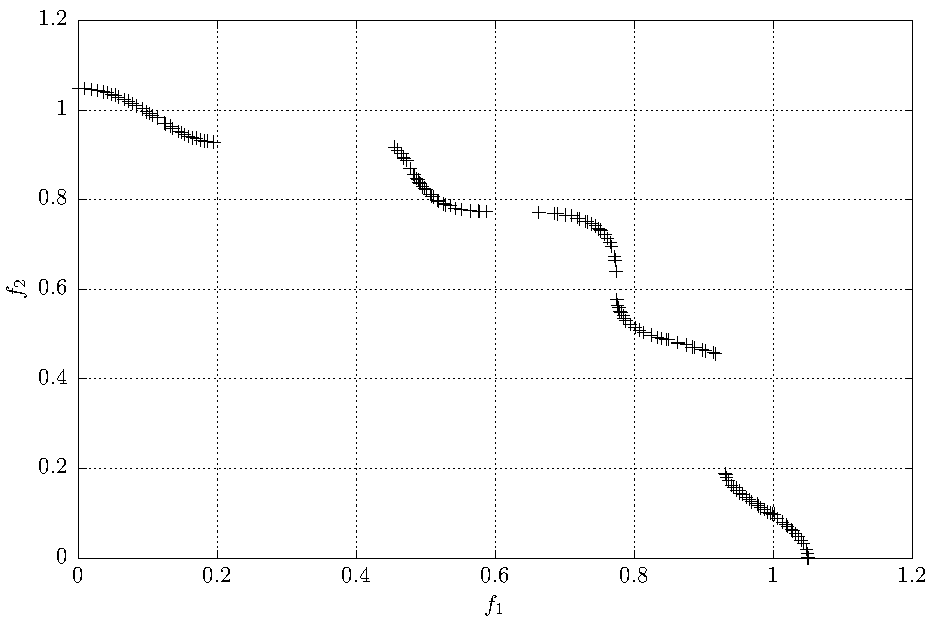
\includegraphics[width=7cm]{tanaka1.pdf}
\caption{Frente de Pareto para el problema de Tanaka semilla 1.}
\label{fig:tanaka1}
\end{figure}

\begin{figure}[hbtp]
\centering
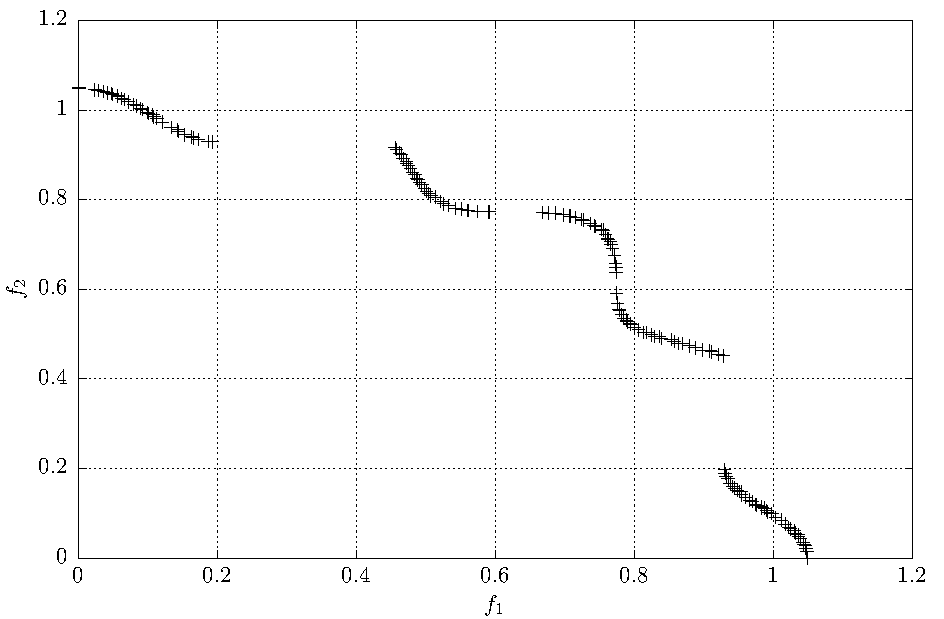
\includegraphics[width=7cm]{tanaka2.pdf}
\caption{Frente de Pareto para el problema de Tanaka semilla 2.}
\label{fig:tanaka2}
\end{figure}

\begin{figure}[hbtp]
\centering
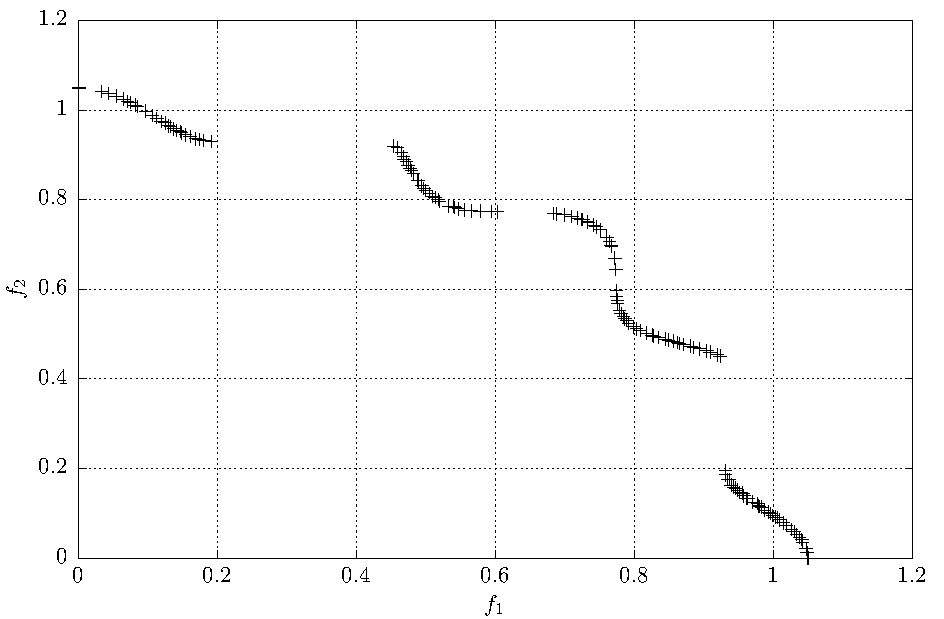
\includegraphics[width=7cm]{tanaka3.pdf}
\caption{Frente de Pareto para el problema de Tanaka semilla 3.}
\label{fig:tanaka3}
\end{figure}



\subsection{Solución de problema de  Osyczka-Kundu}

Para resolver este problema se utilizaron las semillas mostradas en la Tabla \ref{tab:osy} y los siguientes parámetros:

\begin{table}[h!]   
	\caption{Semillas para el algoritmo de Osyczka-Kundu.}                                                                                                                
		\centering                                       
		\begin{tabular}{cc}
			\hline                                             
			Semilla & Valor \\                     
			\hline 
			1 & 0.123\\                                            
			2 & 0.4\\
			3 & 0.5\\
			\hline                                             
		\end{tabular}
		\label{tab:osy}
	\end{table}

\begin{itemize}
\item Tamaño de población: 200
\item Número de generaciones: 250
\item Número de objetivos: 2
\item Número de restricciones: 6
\item Número de variables reales: 6
\item Rango de la variable $x_{1}$: $[ 0, 10]$
\item Rango de la variable $x_{2}$:  $[ 0, 10]$
\item Rango de la variable $x_{3}$: $[ 1, 5]$
\item Rango de la variable $x_{4}$:  $[ 0, 6]$
\item Rango de la variable $x_{5}$: $[ 1, 5]$
\item Rango de la variable $x_{6}$:  $[ 0, 10]$
\item Probabilidad de cruza: 0.9
\item Probabilidad de mutación: 0.1667
\item Índice de distribución para el cruce SBX variable real $\eta_{c}$: 5
\item Índice de distribución para la mutación polinomial variable real $\eta_{m}$: 5
\item Número de variables binarias: 0
\end{itemize}


En las Figuras \ref{fig:tanaka1}, \ref{fig:tanaka2}, \ref{fig:tanaka3} se muestran los frentes de Pareto obtenidos con las semillas de la Tabla \ref{tab:osy}.	
	
\begin{figure}[hbtp]
\centering
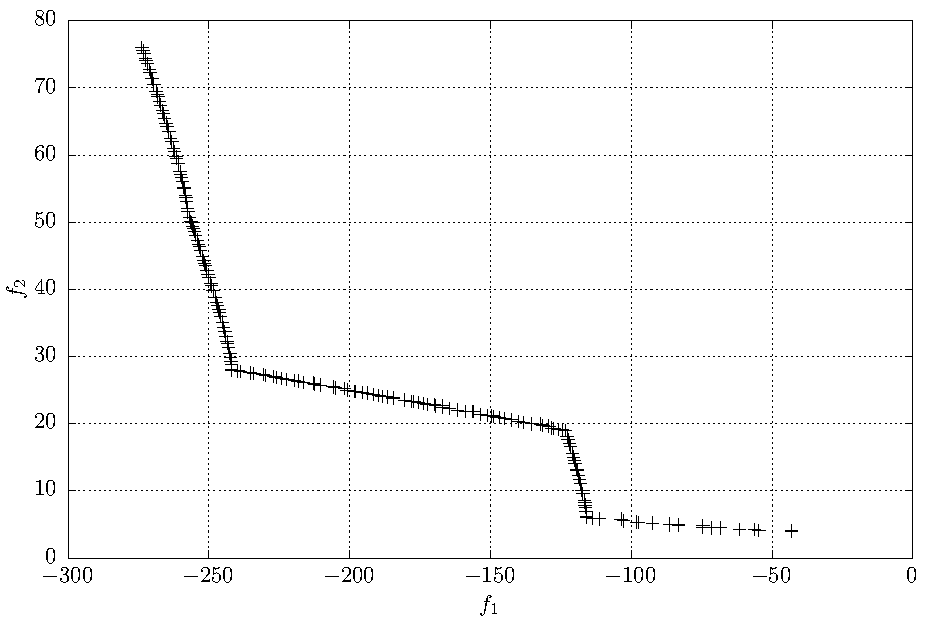
\includegraphics[width=7cm]{osy1.pdf}
\caption{Frente de Pareto para el problema de Osyczka-Kundu semilla 1.}
\label{fig:osy1}
\end{figure}

\begin{figure}[hbtp]
\centering
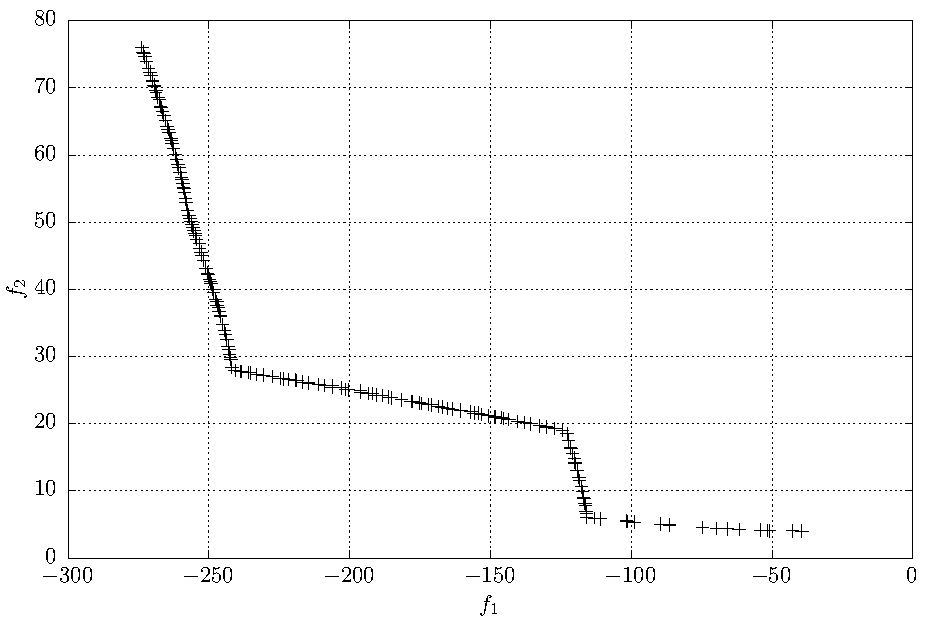
\includegraphics[width=7cm]{osy2.pdf}
\caption{Frente de Pareto para el problema de Osyczka-Kundu semilla 2.}
\label{fig:osy2}
\end{figure}

\begin{figure}[hbtp]
\centering
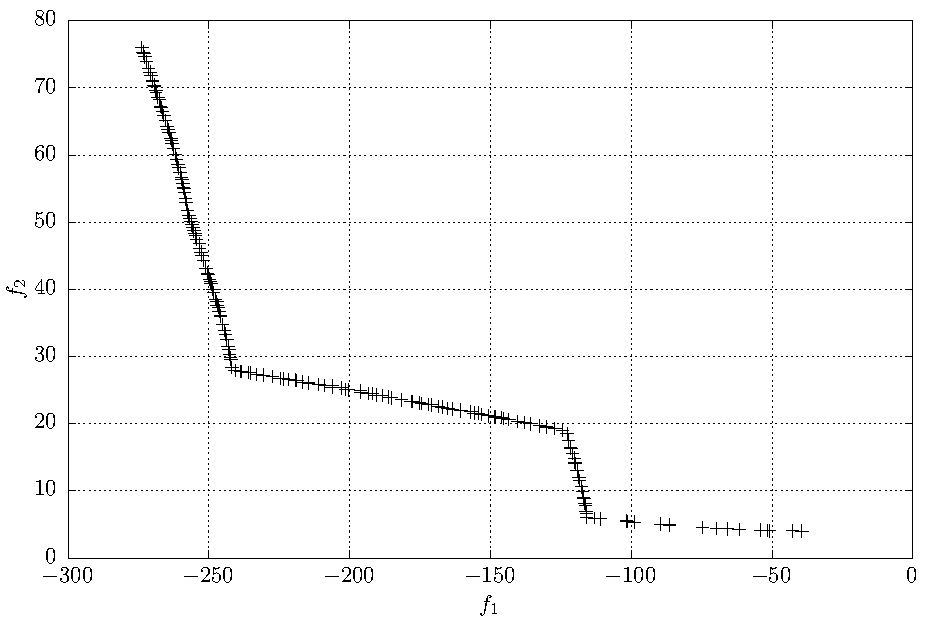
\includegraphics[width=7cm]{osy2.pdf}
\caption{Frente de Pareto para el problema de Osyczka-Kundu semilla 3.}
\label{fig:osy3}
\end{figure}

\section{Conclusiones}

En \cite{b2}, en especifico en las paginas [349 - 352] se presentan ejemplos de los frentes de Pareto para los dos problemas prestados en las secciones anteriores, y los resultados obtenidos coinciden con los frentes de Pareto obtenidos con el algoritmo NSGA-II. Es importante resaltar que el frente de Pareto nos indica cuales son las soluciones que cumplen tanto con las funciones objetivo como con las restricciones, sin embargo este solo nos da una idea general de las soluciones y es necesario elegir una de ellas dependiendo de las características necesarias, en otras palabras siempre existirá un compromiso al elegir un punto en el frente de Pareto.

De mismo modo es importante resaltar la eficiencia del algoritmo, el tiempo de ejecución en muy bajo debido a su codificación en C y en rasgos generales es sencillo de utilizar con la única complicación de tener que elegir manualmente los parámetros de cruza y mutación.


\begin{thebibliography}{00}
\bibitem{b1}  Dr. Luis Gerardo de la Fraga. ``Apuntes de clase'' .
\bibitem{b2} Kalyanmoy Deb.``Multi-objetive Optimization using Evolutionary Algoritms'', John Wiley, 1ra Ed.
\end{thebibliography}


\end{document}
